\documentclass[12pt,a4paper]{article}
\usepackage[english,russian]{babel} 

\usepackage{cmap}
\usepackage{hyperref}
\usepackage{xcolor}
\definecolor{linkcolor}{HTML}{0000FF}
\definecolor{urlcolor}{HTML}{FF0000}

\usepackage{amsfonts}
 
\hypersetup{pdfstartview=FitH,  linkcolor=linkcolor,urlcolor=urlcolor, colorlinks=true}
\usepackage{hyphenat}
\usepackage{graphicx}
\usepackage[intlimits]{amsmath}
\usepackage{amssymb}
\usepackage{amsmath}
\usepackage{mathtools}
\usepackage{minted}

\title{poseDesignerDoc}
\author{Смирнов Иван }
\date{August 2022}

\begin{document}

\tableofcontents
\newpage

\section{Описание функционала}
\subsection{меню File}
\label{file}
\begin{figure}[h!]
    \centering
    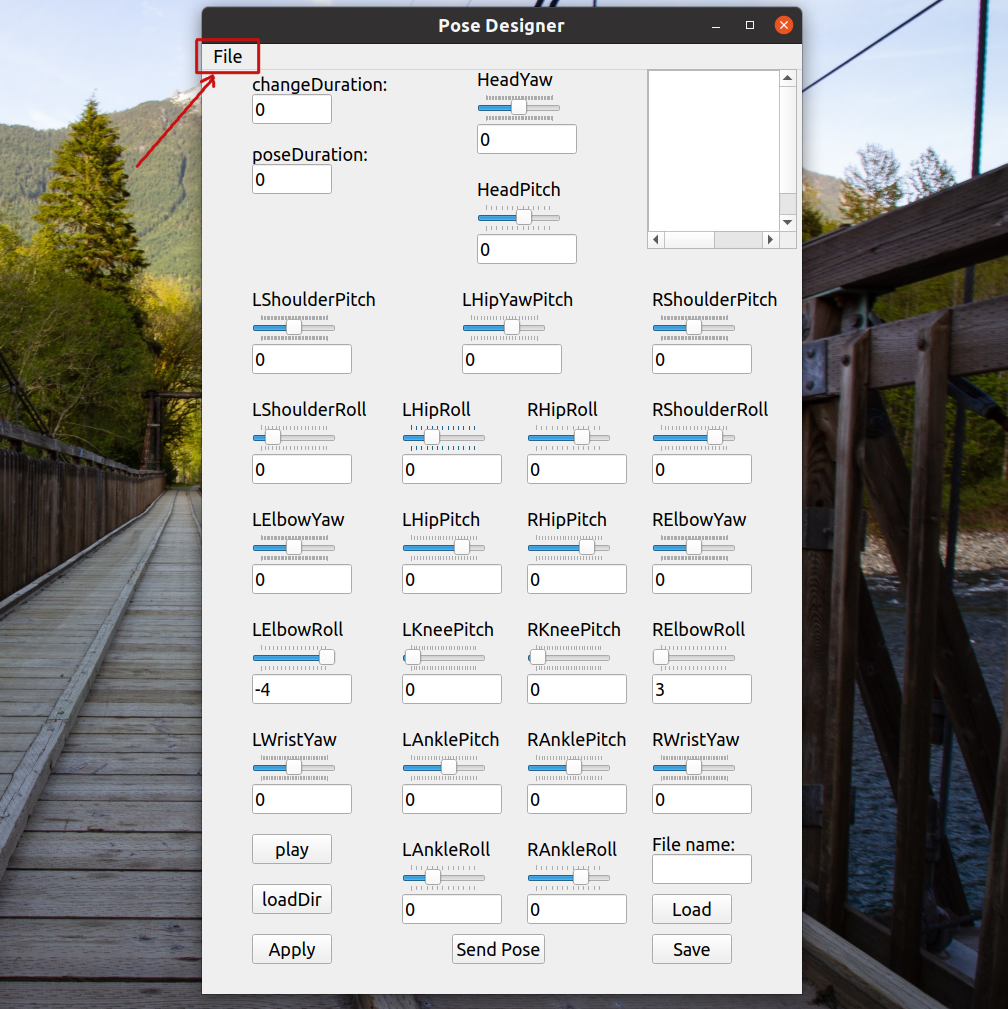
\includegraphics[width=0.99\textwidth]{images/file.png}
    \caption{Меню File располагается в верхнем левом углу окна приложения. С его помощью[single click] можно открыть меню, предлагающее выбрать папки для сохранения и загрузки поз. В появившемся меню одиночным нажатием ЛКМ можно перейти к окошку выбора соответствуюшей директории.}
    \label{fig:file}
\end{figure}
\newpage
\subsection{Scroll area}
\label{scroll}
\begin{figure}[h!]
    \centering
    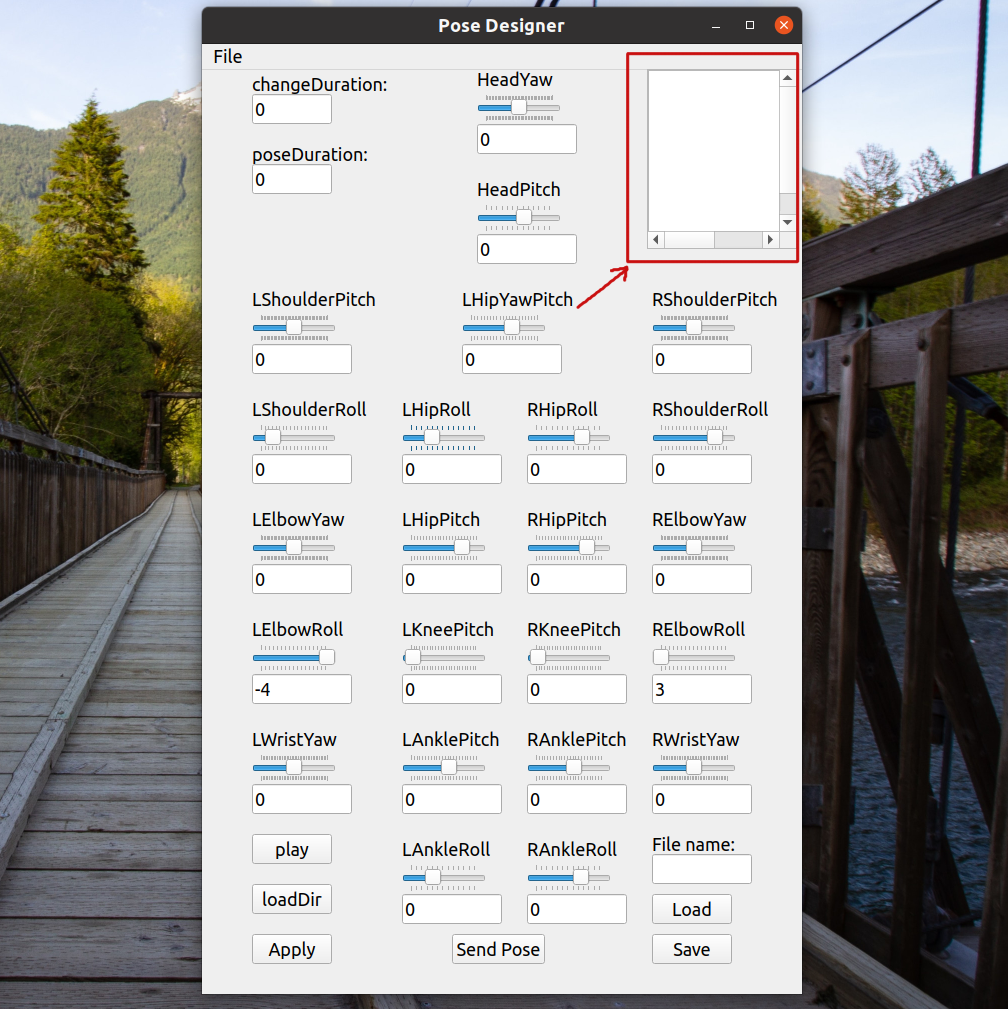
\includegraphics[width=0.99\textwidth]{images/scroll.png}
    \caption{Область прокрутки располагается в правом верхнем углу. В ней отображаются файлы(позы) в выбранной папке \italic{load directory} после нажатия на \hyperref[loadDir]{кнопку loadDir}. После двойного щелчка ЛКМ на позу в этой области, она отобразится на \hyperref[sliders]{слайдерах} и \hyperref[durations]{окошках длительностей} }
    \label{fig:file}
\end{figure}
\newpage
\subsection{Кнопки}
\subsubsection{save, load}
\label{saveLoad}
\begin{figure}[h!]
    \centering
    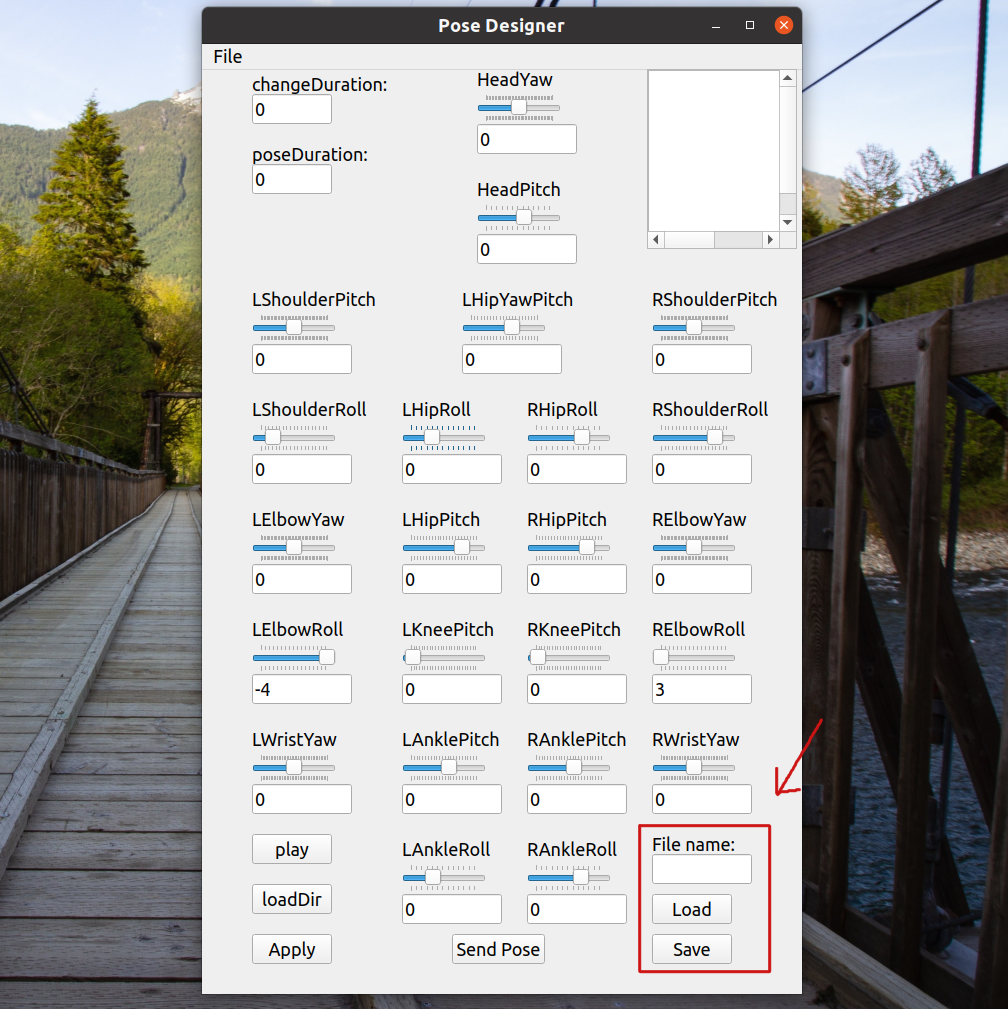
\includegraphics[width=0.99\textwidth]{images/loadSave.png}
    \caption{Кнопки для сохранения и загрузки, а также окно ввода "File name". При необходимости выполняют сохранение и загрузку файла с именем в окне ввода(по умолчанию "pose.txt") из \hyperref[file]{дирректорий сохранения и ввода соответственно} в \hyperref[messageView]{оговоренном формате}.}
    \label{fig:file}
\end{figure}
\newpage
\subsubsection{loadDir}
\label{loadDir}
\begin{figure}[h!]
    \centering
    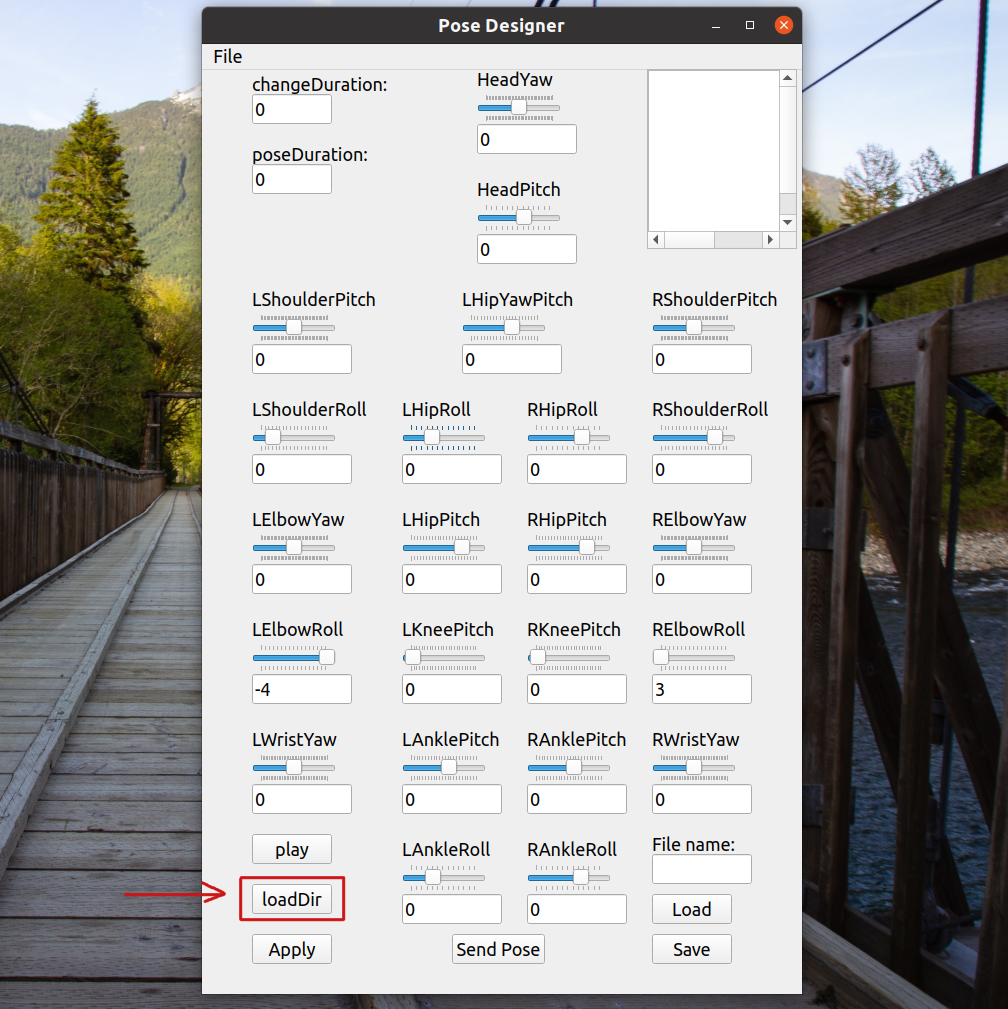
\includegraphics[width=0.99\textwidth]{images/loadDir.png}
    \caption{Нажатие на эту кнопку обновляет \hyperref[scroll]{область прокрутки с файлами для проигрывания} согласно файлам в \hyperref[file]{директории для загрузки}(по умолчанию точка запуска приложения - ros workspace).}
    \label{fig:file}
\end{figure}
\newpage
\subsubsection{apply}
\label{apply}
\begin{figure}[h!]
    \centering
    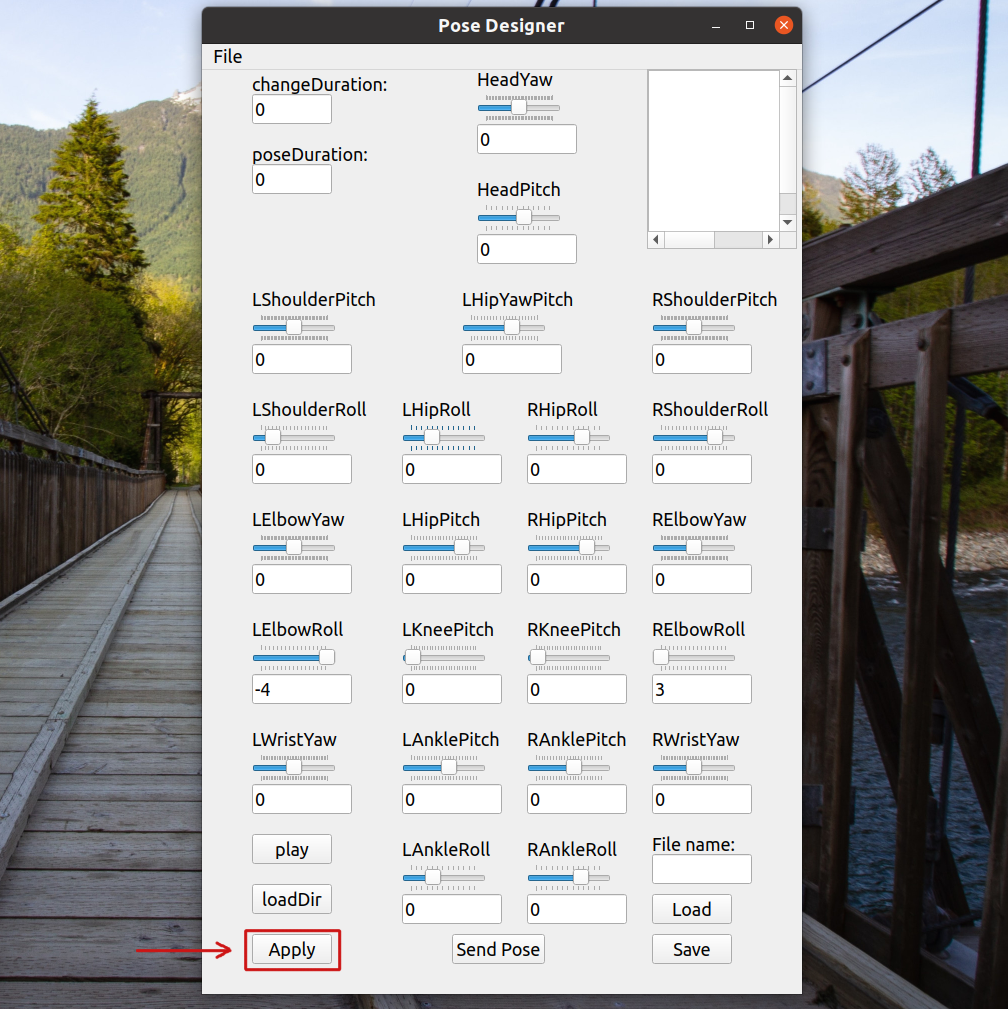
\includegraphics[width=0.99\textwidth]{images/apply.png}
    \caption{Нажатие на эту кнопку согласует подписи в окошках под слайдерами с их положением. Без этого действия изменения, внесённые в слайдеры по средством окошек под ними не являются учтёнными приложением.}
    \label{fig:file}
\end{figure}
\newpage
\subsubsection{sendPose}
\label{sendPose}
\begin{figure}[h!]
    \centering
    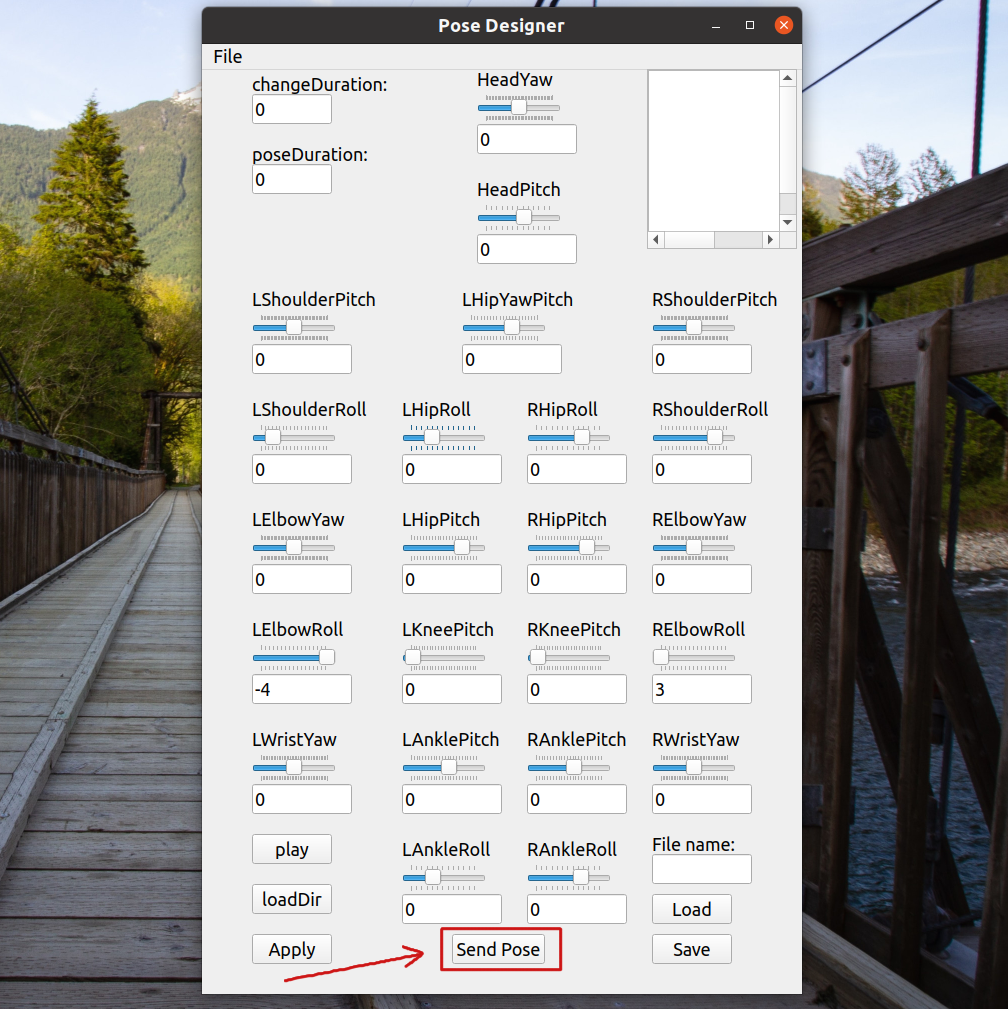
\includegraphics[width=0.99\textwidth]{images/sendPose.png}
    \caption{Отпрвка текущего состояния(позии соединений - моторов и продолжительности) на робота(в топик effectors/joint\_positions, с одновременной отправкой в effectors/joint\_stifnesses едениц для каждого соединения-мотора).}
    \label{fig:file}
\end{figure}
\newpage
\subsubsection{play}
\label{play}
\begin{figure}[h!]
    \centering
    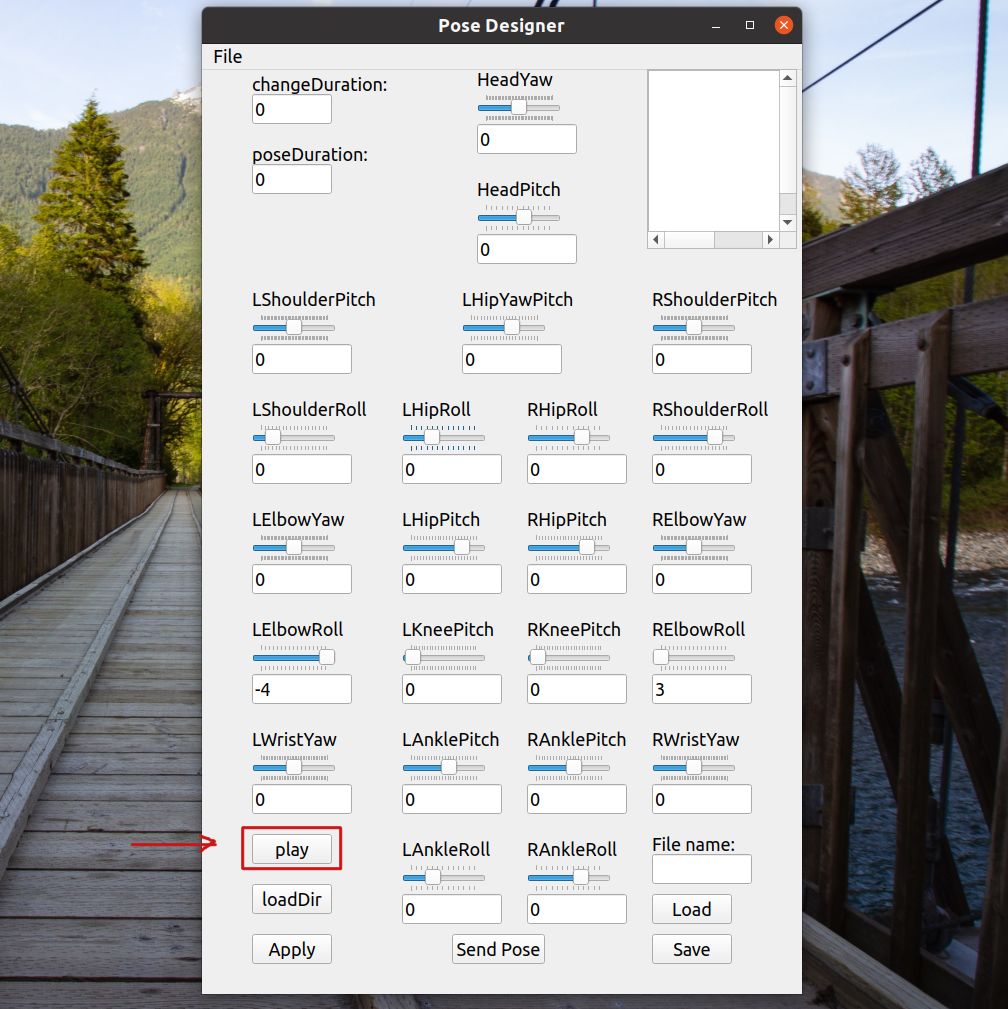
\includegraphics[width=0.99\textwidth]{images/play.png}
    \caption{Нажатие на эту кнопку осуществляет последовательную отправку поз-состояний на робота(порядок отправки агалогичен кнопки \hyperref[sendPose]{обычной отправки}) из списка \hyperref[scroll]{области прокрутки}, также учитываются продолжительности.}
    \label{fig:file}
\end{figure}
\newpage
\subsection{окошки durations}
\label{durations}
\begin{figure}[h!]
    \centering
    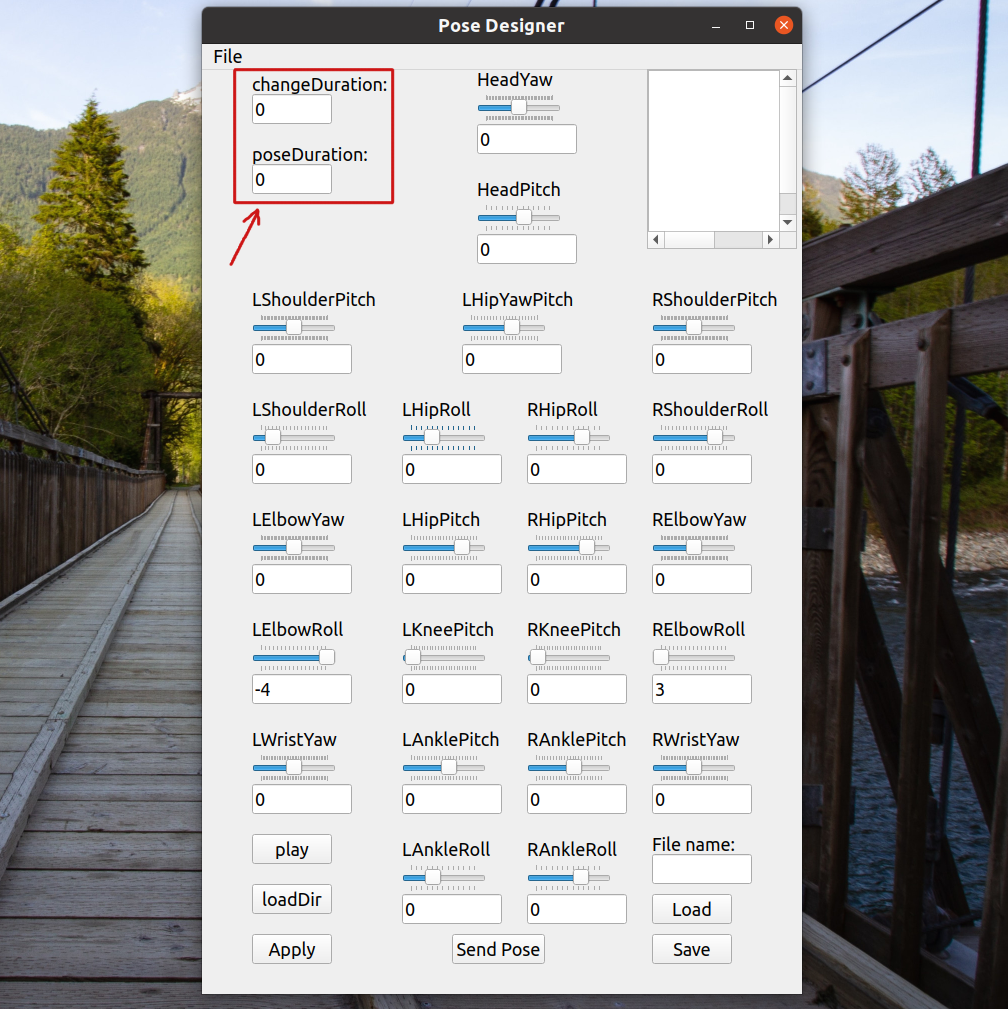
\includegraphics[width=0.99\textwidth]{images/durations.png}
    \caption{Окошки для ввода длительностей находятся в левом верхнем углу, чуть ниже \hyperref[file]{меню file}. \italic{changeDuration} - продолжительность[ms] перехода в следующее положение(позу), \italic{poseDuration} - продолжительность[ms] пребывания в данной позе. В качестве значений используются числа из множества $\{0\} \vee \mathbf{N}$. Робот Nao v6 может выполнять команды каждые $12ms$, соответственно необходимо это учитывать при выставлении данных полей. По умолчанию они инициализированны нулями. }
    \label{fig:file}
\end{figure}
\newpage
\subsection{Слайдеры}
\label{sliders}
Основной функционал данного приложения представляют многочисленные слайдеры. С их помощью можно выставлять значения для конкретного соединения(\italic{joint}).
\begin{itemize}
    \item Допустимые значения взяты из официального \href{http://doc.aldebaran.com/2-8/family/nao_technical/joints_naov6.html}{официального сайта} c небольшим запасом[1 - 2 градуса].
    \item Начальные положения выставляются в соответствии с начальным положением робота при стойке с вытянутыми руками.
    \item Учтены зависимости соединений. То есть тот факт, что область допустимых значений некоторых соединений меняется в зависимости от остальных соединений.
    \end{itemize}
Поэтому гарантированно с помощью данного приложения нельзя создать физически не реализуеммую позу.\\
Также помимо слайдеров можно использовать и окошки под ними, в которые стоит выставлять значения угла в градусах из диапозона $(\{0\} \vee \mathbf{N})$, не стоит беспокоится о неверных значениях, так как при нажатии \hyperref[apply]{кнопки apply} происходит автоматическая проверка значений, выставленных в окошки слайдеров. \textbf{Нажатие данной кнопки обязательно} для считывания приложением значений из этих окошек(при отсутствии нажатия, учёта этих значений не будет).
\newpage
\section{Возможный сценарий работы}
\subsection{Запуск мира в Webots}
Первым дело необходимо запустить мир с роботом Nao в Webots. Для этого в открытом приложении Webots жмём \italic{File->Open World}. В открывшемся окне выбираем \italic{WebotsLoLa->worlds->nao\_robocup.wbt}. После этого в приложении Webots должно появится \hyperref[fig:world]{следующее}.
\begin{figure}[h!]
    \centering
    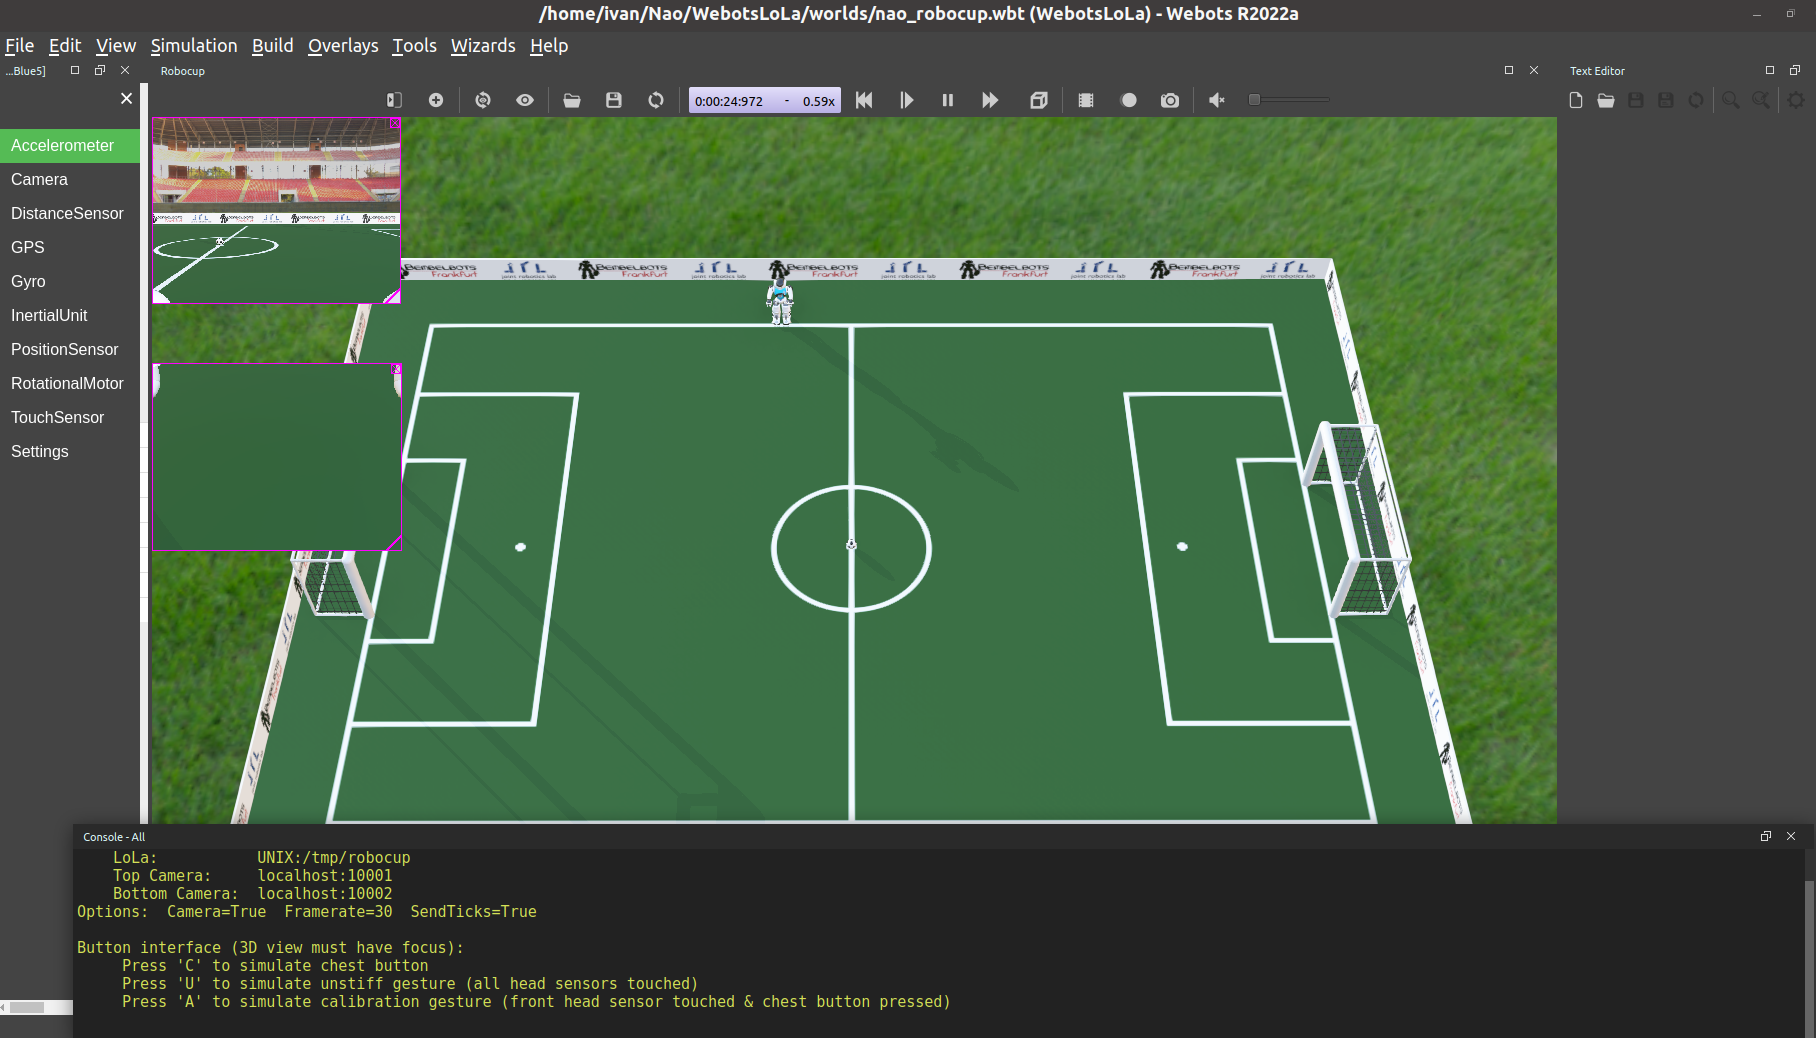
\includegraphics[width = 0.99\textwidth]{./images/webotsWorldOpen.png}
    \caption{Открытие мира с роботом Nao в Webots.}
    \label{fig:world}
\end{figure}
\newpage
\subsection{Включение nao\_lola}
Для осуществления связи робота в Webots с приложением pose\_design используется ROS2 node nao\_lola. Её можно запустить в терминале при помощи команды:\\
\begin{minted}{python}
ros2 run nao_lola nao_lola
\end{minted}
После этого результат соединения Webots с nao\_lola отобразится в левом нижнем углу терминала \hyperref[fig:webotsNaoLola]{Webots} с сообщением зелёного цвета \italic{Lola client connected}.
\begin{figure}[h!]
    \centering
    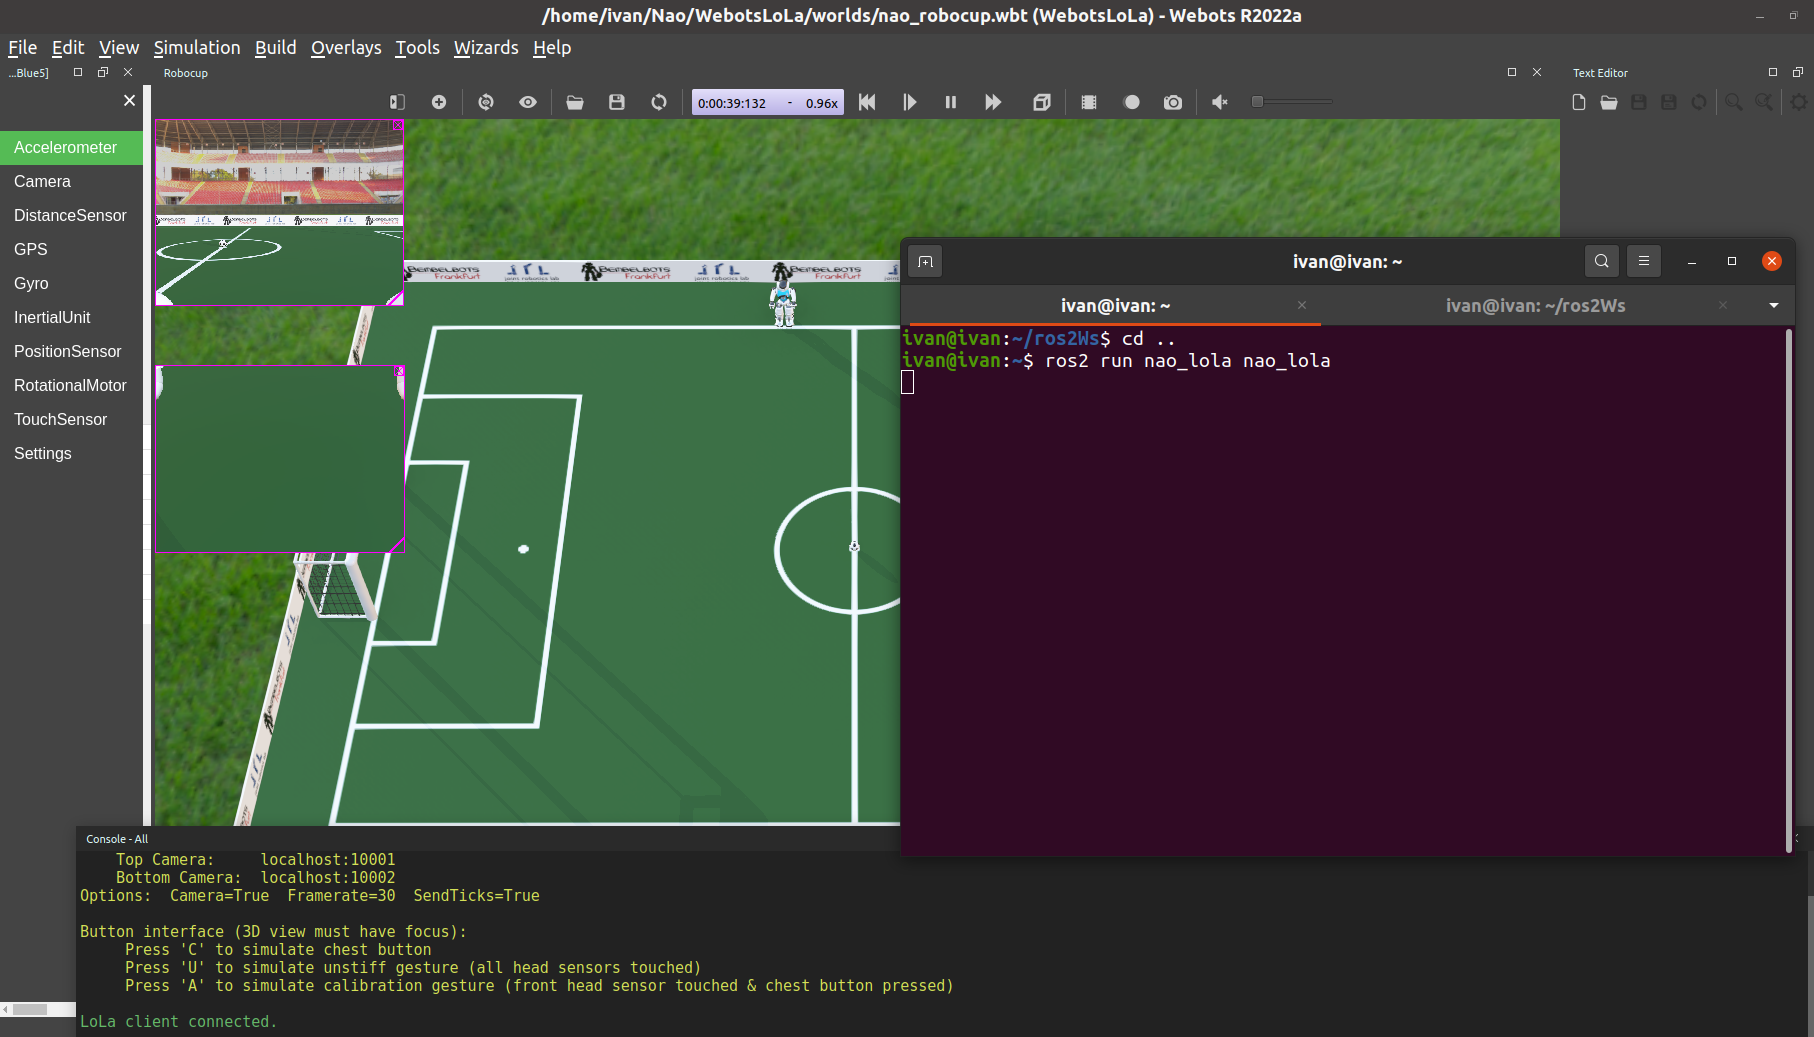
\includegraphics[width = 0.99\textwidth]{./images/webotsNaoLola.png}
    \caption{Запуск ROS2 node nao\_lola, и соединение с Webots.}
    \label{fig:webotsNaoLola}
\end{figure}
\newpage
\subsection{Включение приложение pose\_design}
Само приложение представляет из себя тоже ROS2 node с графическим интерфейсом, поэтому для её запуска необходимо перейти в терминал в \italic{ros2 workspace}, и ввести следующие команды: 
\begin{minted}{python}
. install\setup.bash
ros2 run pose_design pose_design
\end{minted}
В результате откроется \hyperref[fig:pose_design]{приложение}.
\begin{figure}[h!]
    \centering
    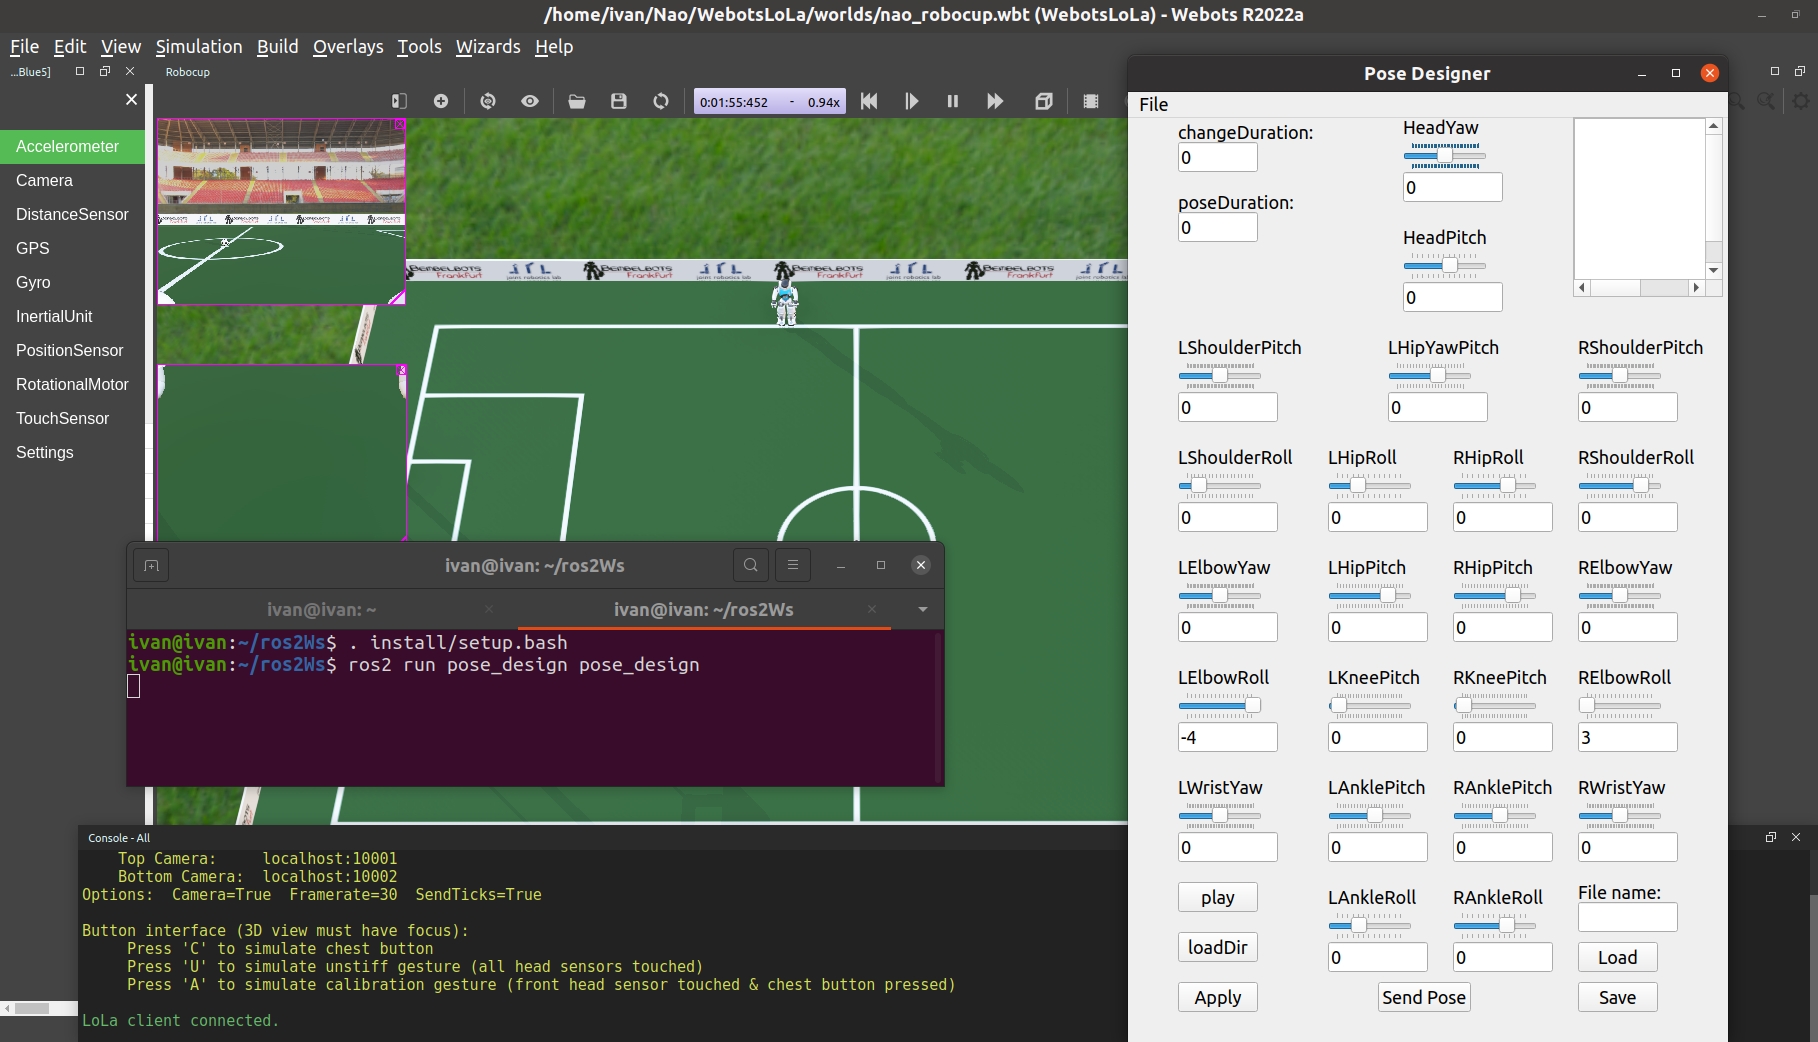
\includegraphics[width = 0.99\textwidth]{./images/webotsPoseDesign.png}
    \caption{Запуск приложения pose\_design.}
    \label{fig:pose_design}
\end{figure}
\newpage
\subsection{Выбор папок загрузки и сохранения}
Перед началом работы с приложением рекомендуется выбрать \hyperref[file]{папки для загрузки и сохранения поз}. Сейчас будет создано несколько поз, а потом они же и проиграны, поэтому папки загрузки и сохранения совпадают(изначально это пустая папка).
\begin{figure}[h!]
    \centering
    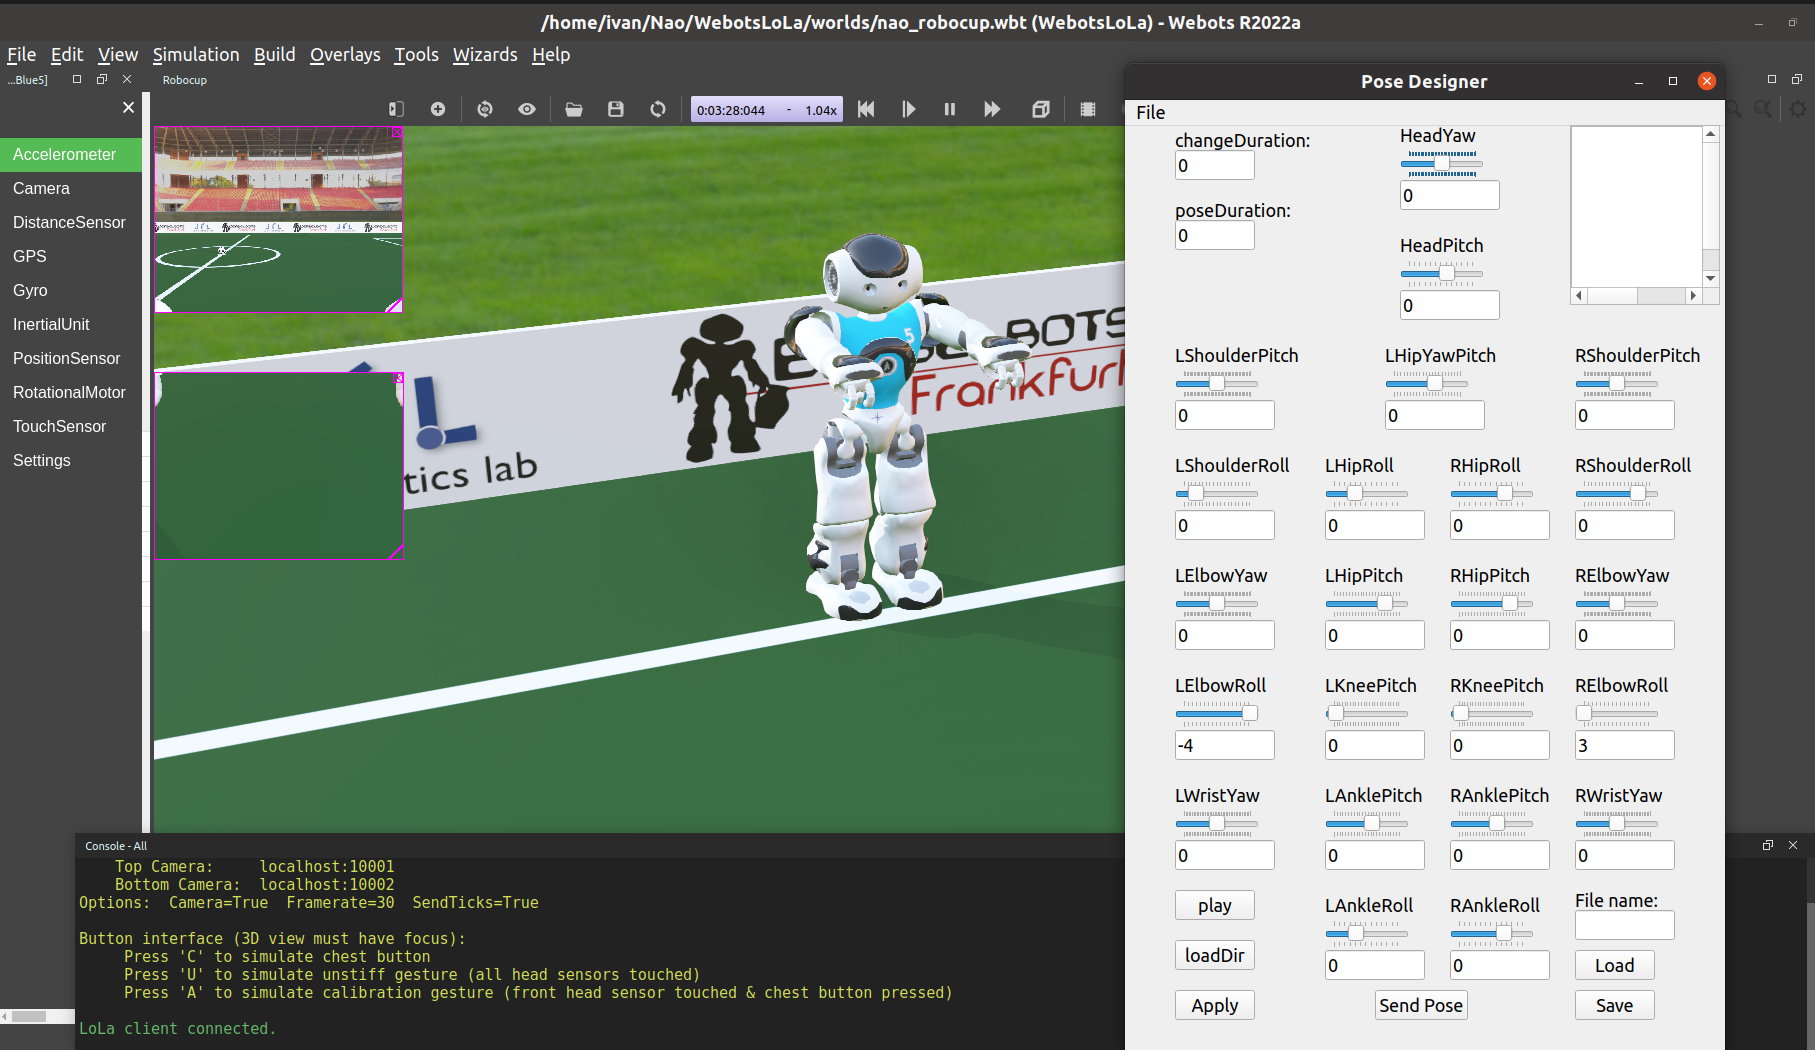
\includegraphics[width = 0.99\textwidth]{./images/webotsDirSelect.png}
    \caption{Выбор папок загрузки и сохранения.}
    \label{fig:webotsDirSelect}
\end{figure}
\newpage
\subsection{Отправка сообщения-позы на робота}
В начале посмотрим как работает кнопка \hyperref[sendPose]{отправки позы на робота}. Для этого выставим какую-то позу отличную от начальной, например поворот головы влево. Затем нажмём на кнопку \hyperref[sendPose]{отправки}. Результат работы можно видедеть на изображении ниже.
\begin{figure}[h!]
    \centering
    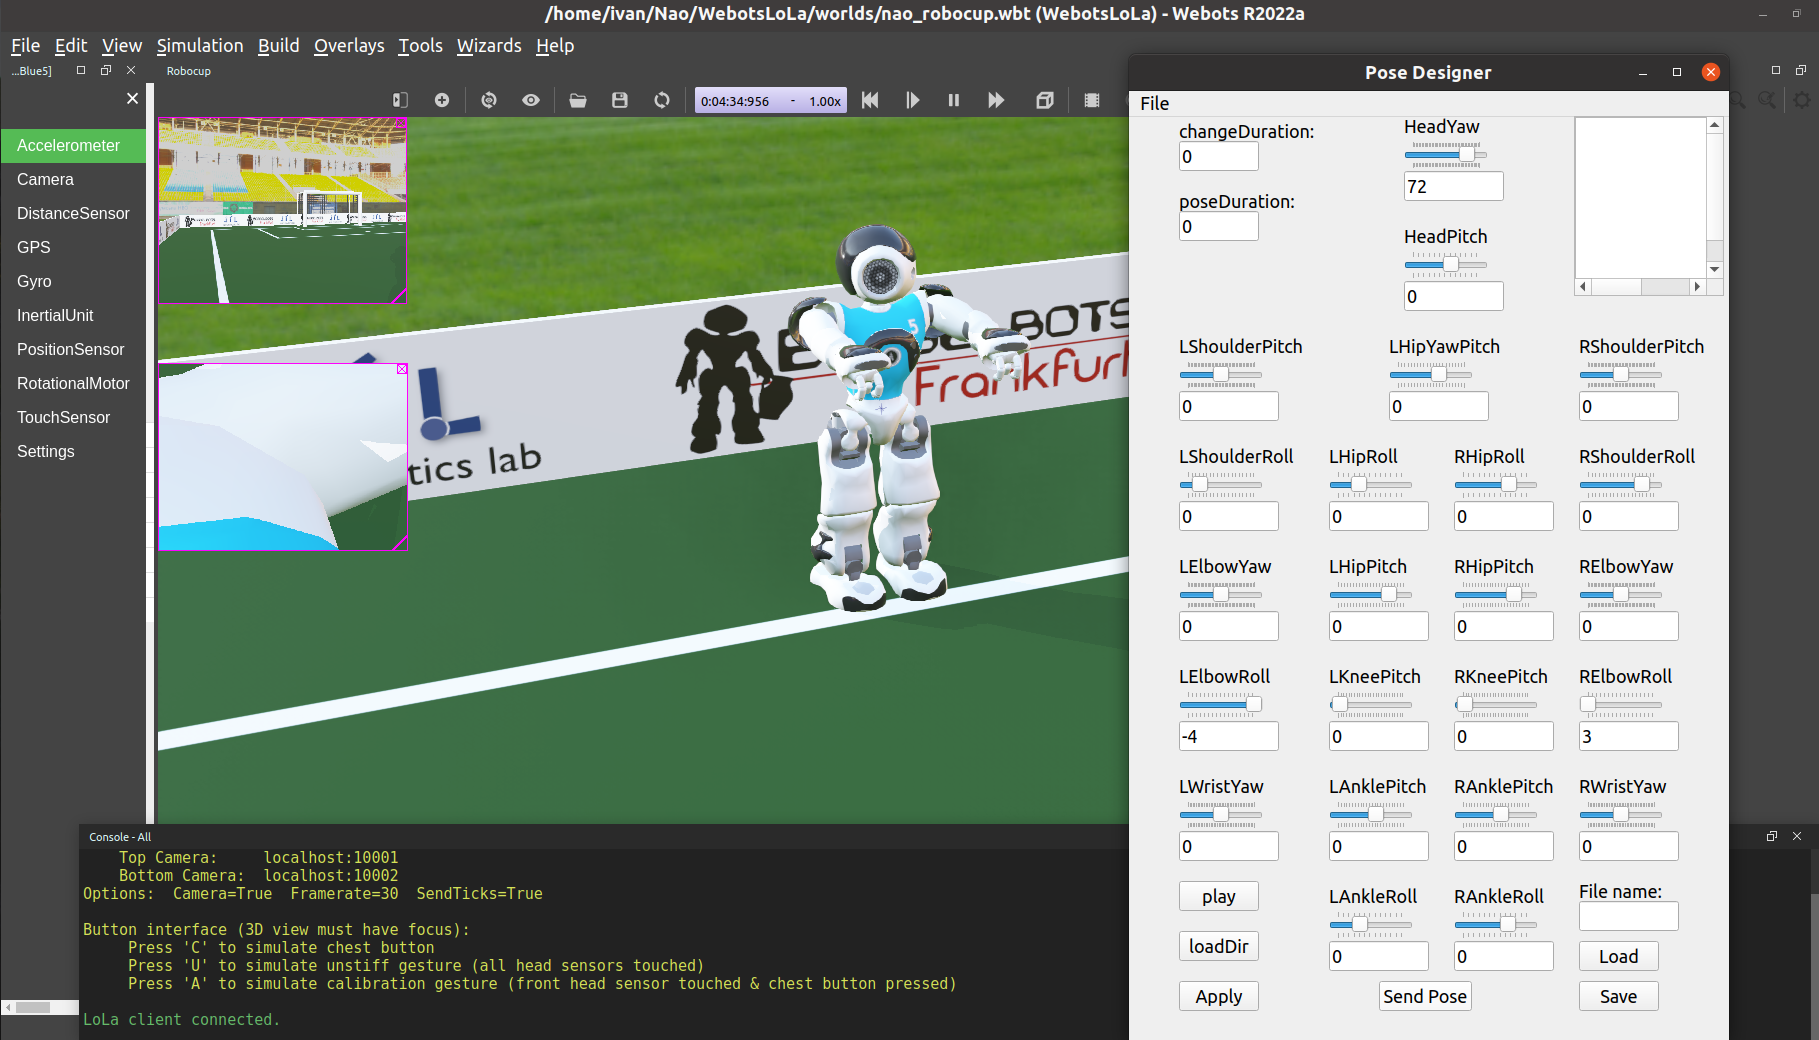
\includegraphics[width = 0.72\textwidth]{./images/firstTurn.png}
    \caption{Отправка позы на робота.}
    \label{fig:my_label}
\end{figure}
\subsection{Сохранение одной позы в файл}
Для сохранения позы используем \hyperref[save]{кнопку сохранения, с окошком ввода имени файла}. Введём например название \itslic{pose1.txt}, и нажмём \italic{Save}. Поза должна появится в папке для сохранения.
\begin{figure}[h!]
    \centering
    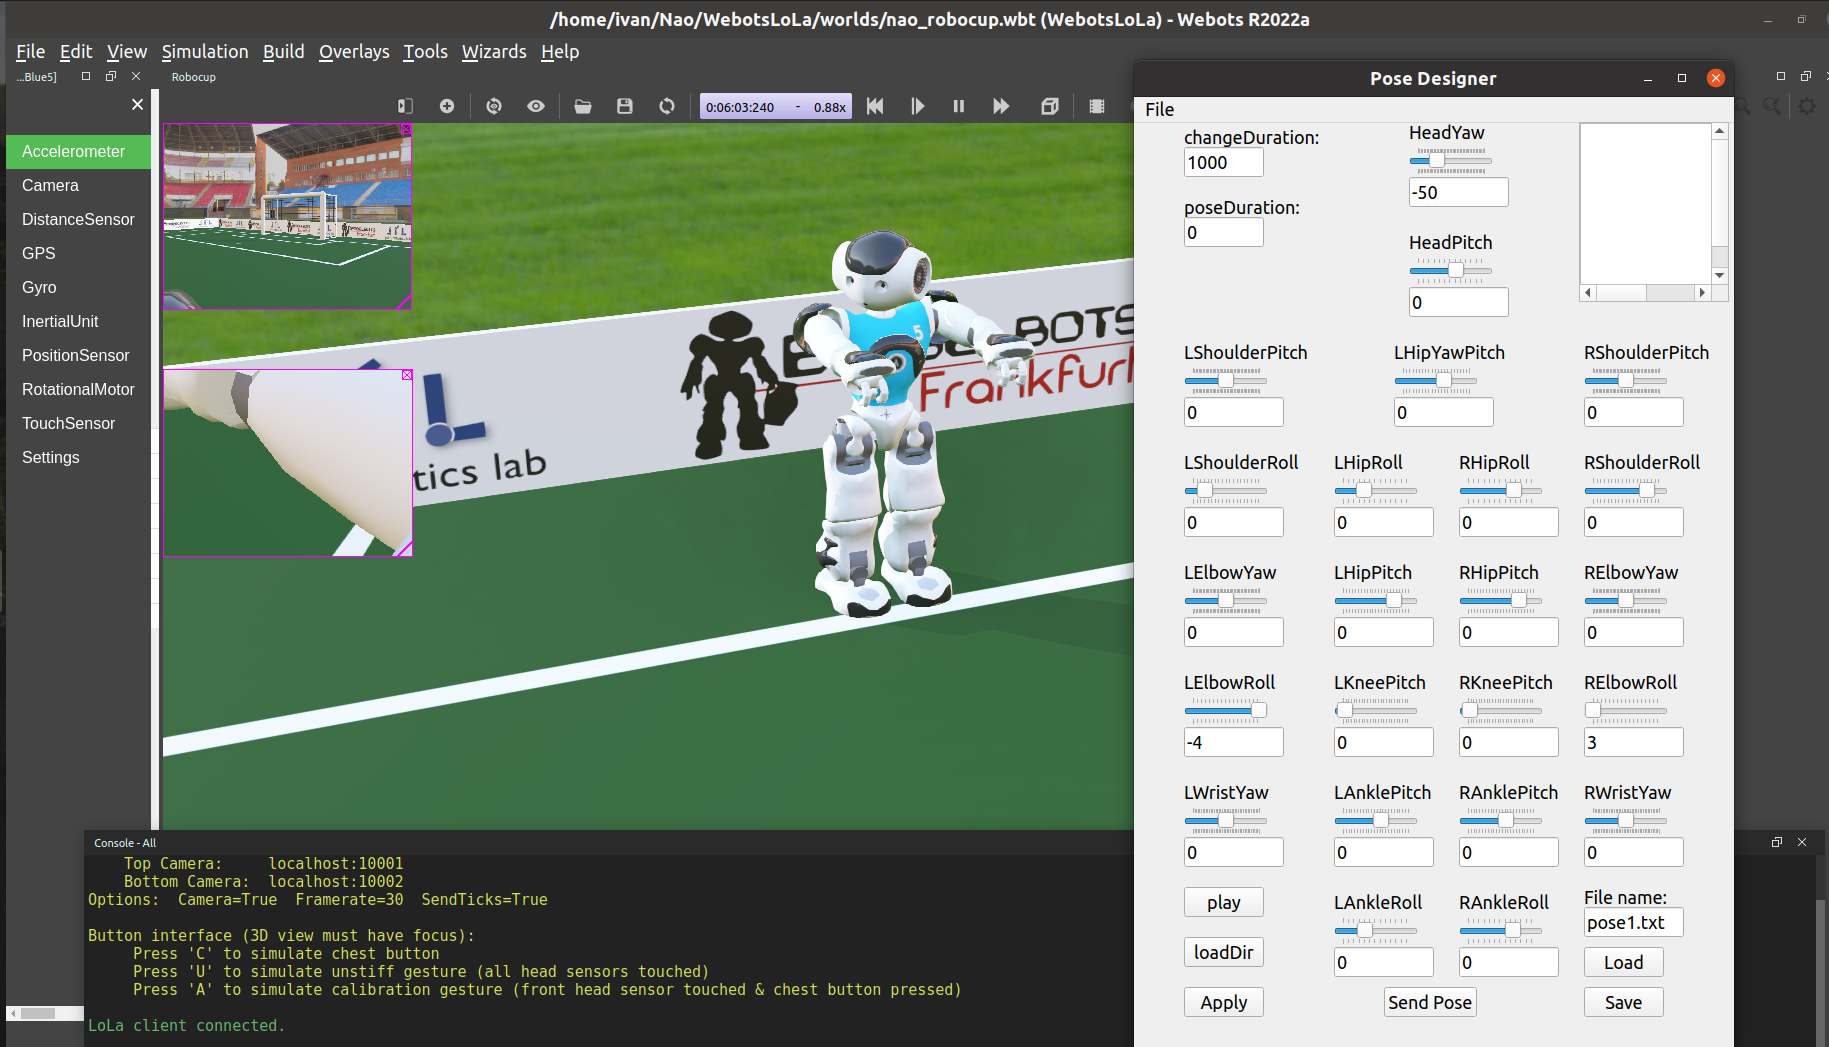
\includegraphics[width = 0.72\textwidth]{./images/firstSave.png}
    \caption{Сохранение позы.}
    \label{fig:my_label}
\end{figure}
\newpage
\subsection{Выставление позы через окно под слайдером}
Также можно выставить позу, например поворот головы вправо, при помощи окна ввода под слайдером. Для этого щёлкаем ЛКМ на окошко под слайдером и выставляем значение(работаем как с обычным полем вводы, то есть можно пользоваться например кнопками стирания текста). Как можно увидеть, слайдер остался на месте.
\begin{figure}[h!]
    \centering
    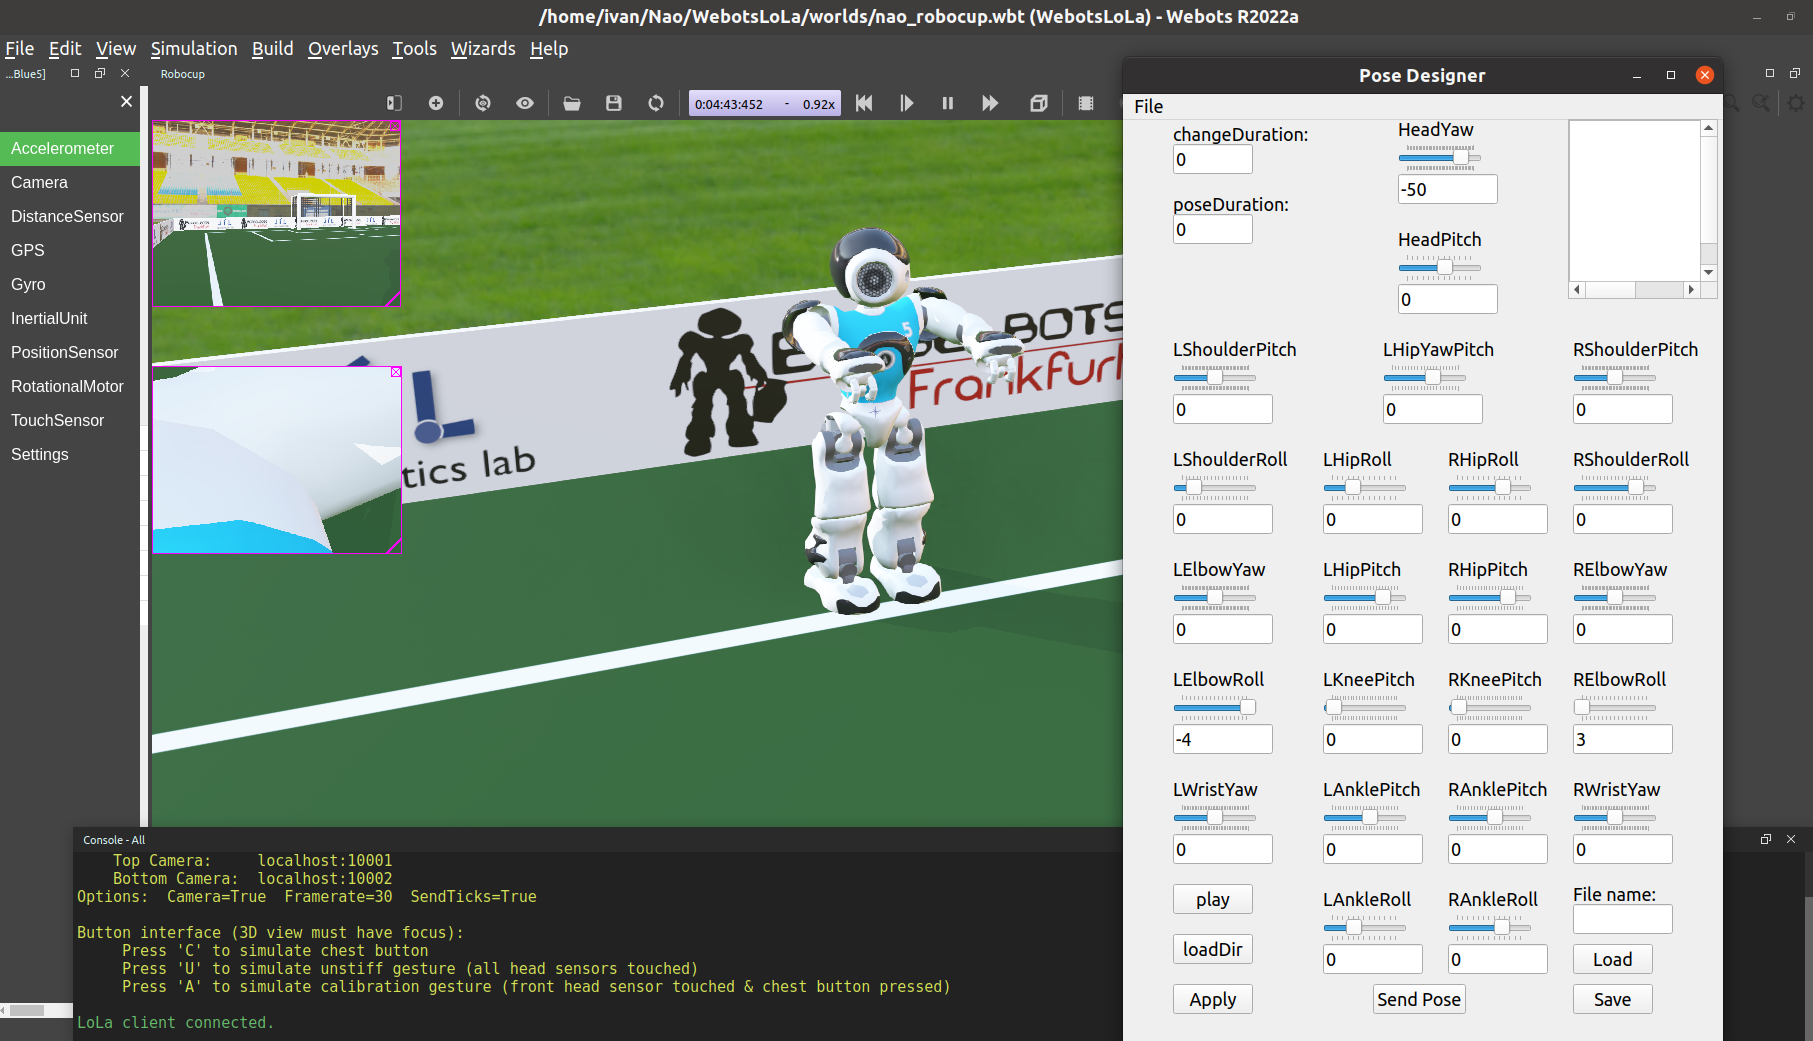
\includegraphics[width = 0.8\textwidth]{./images/sliderChange.png}
    \caption{Ввод значения слацдера в окошко под ним.}
    \label{fig:my_label}
\end{figure}

\noindent Теперь нажмём на \hyperref[apply]{кнопку apply}, и увидим, что слайдер согласовался с значением в окошки под ним.
\begin{figure}[h!]
    \centering
    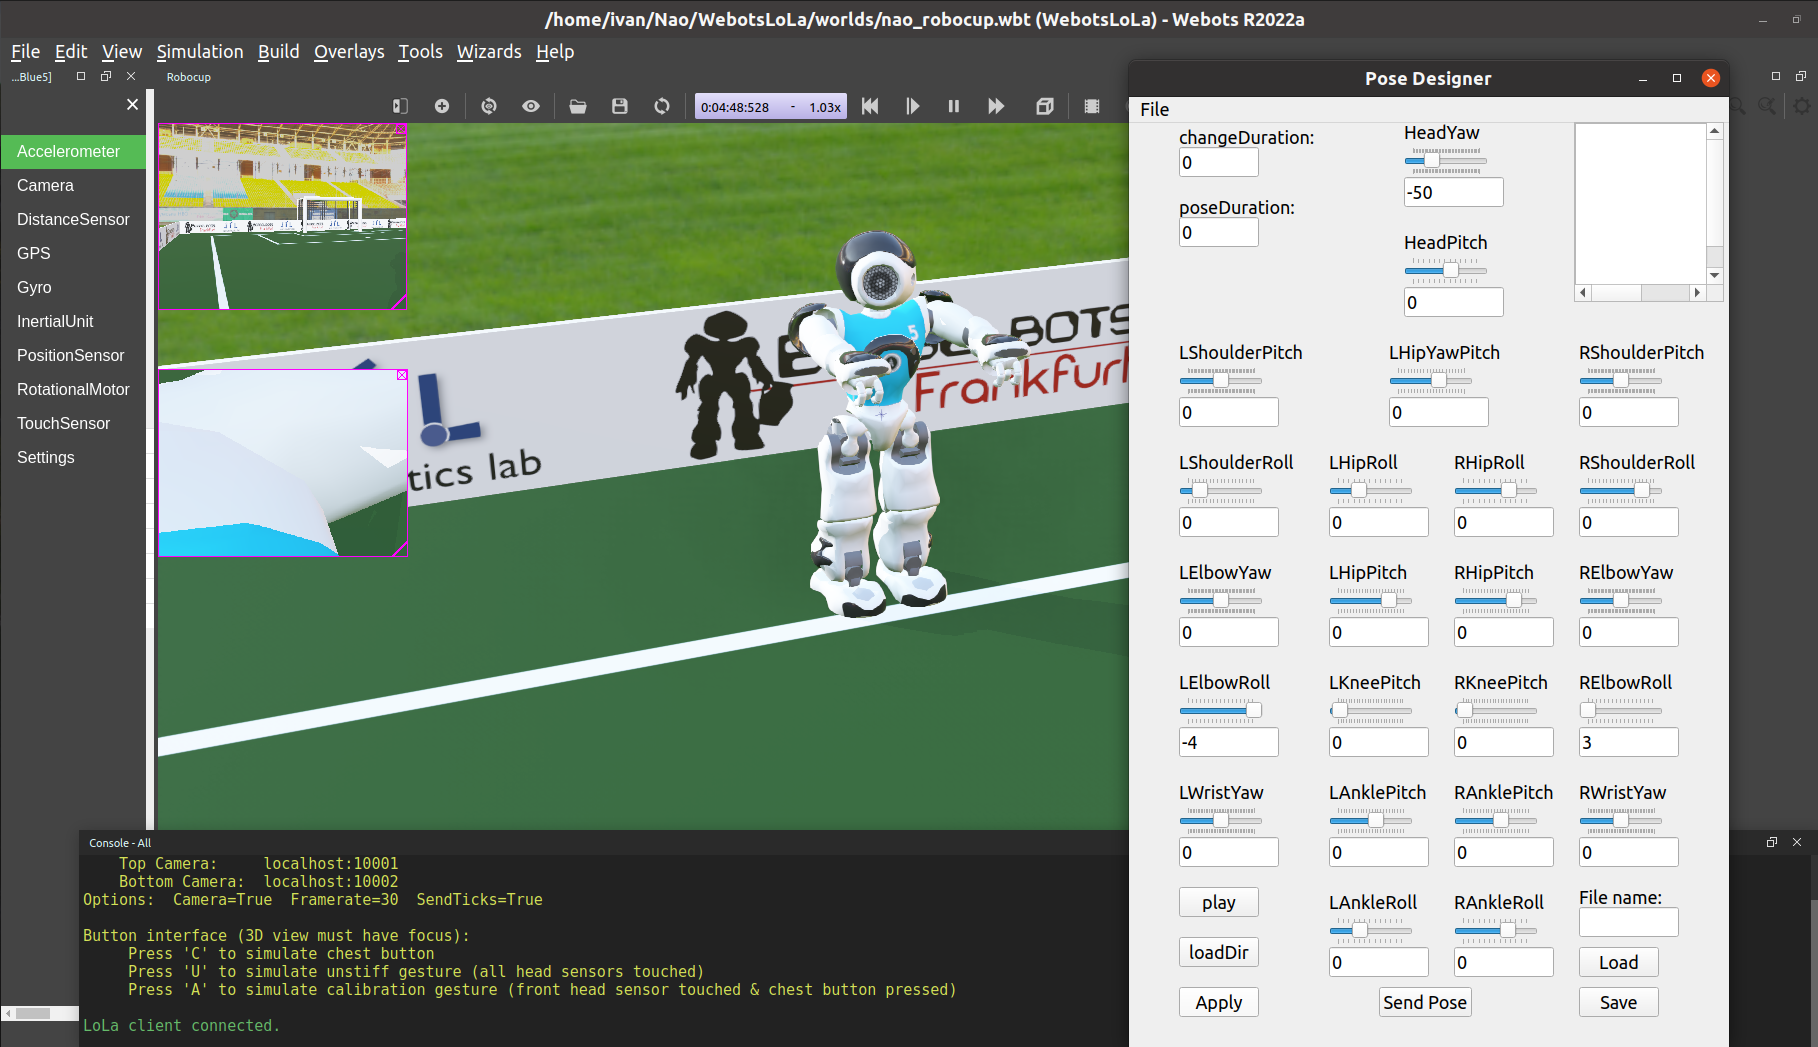
\includegraphics[width = 0.8\textwidth]{./images/applyClick.png}
    \caption{Нажатие \hyperref[apply]{кнопки apply} после выставление слайдера с помощью окошка под ним.}
    \label{fig:my_label}
\end{figure}
\newpage
\noindent Отправим позу на робота, при помощи уже \hyperref[sendPose]{изученной кнопки отправки}.
\begin{figure}[h!]
    \centering
    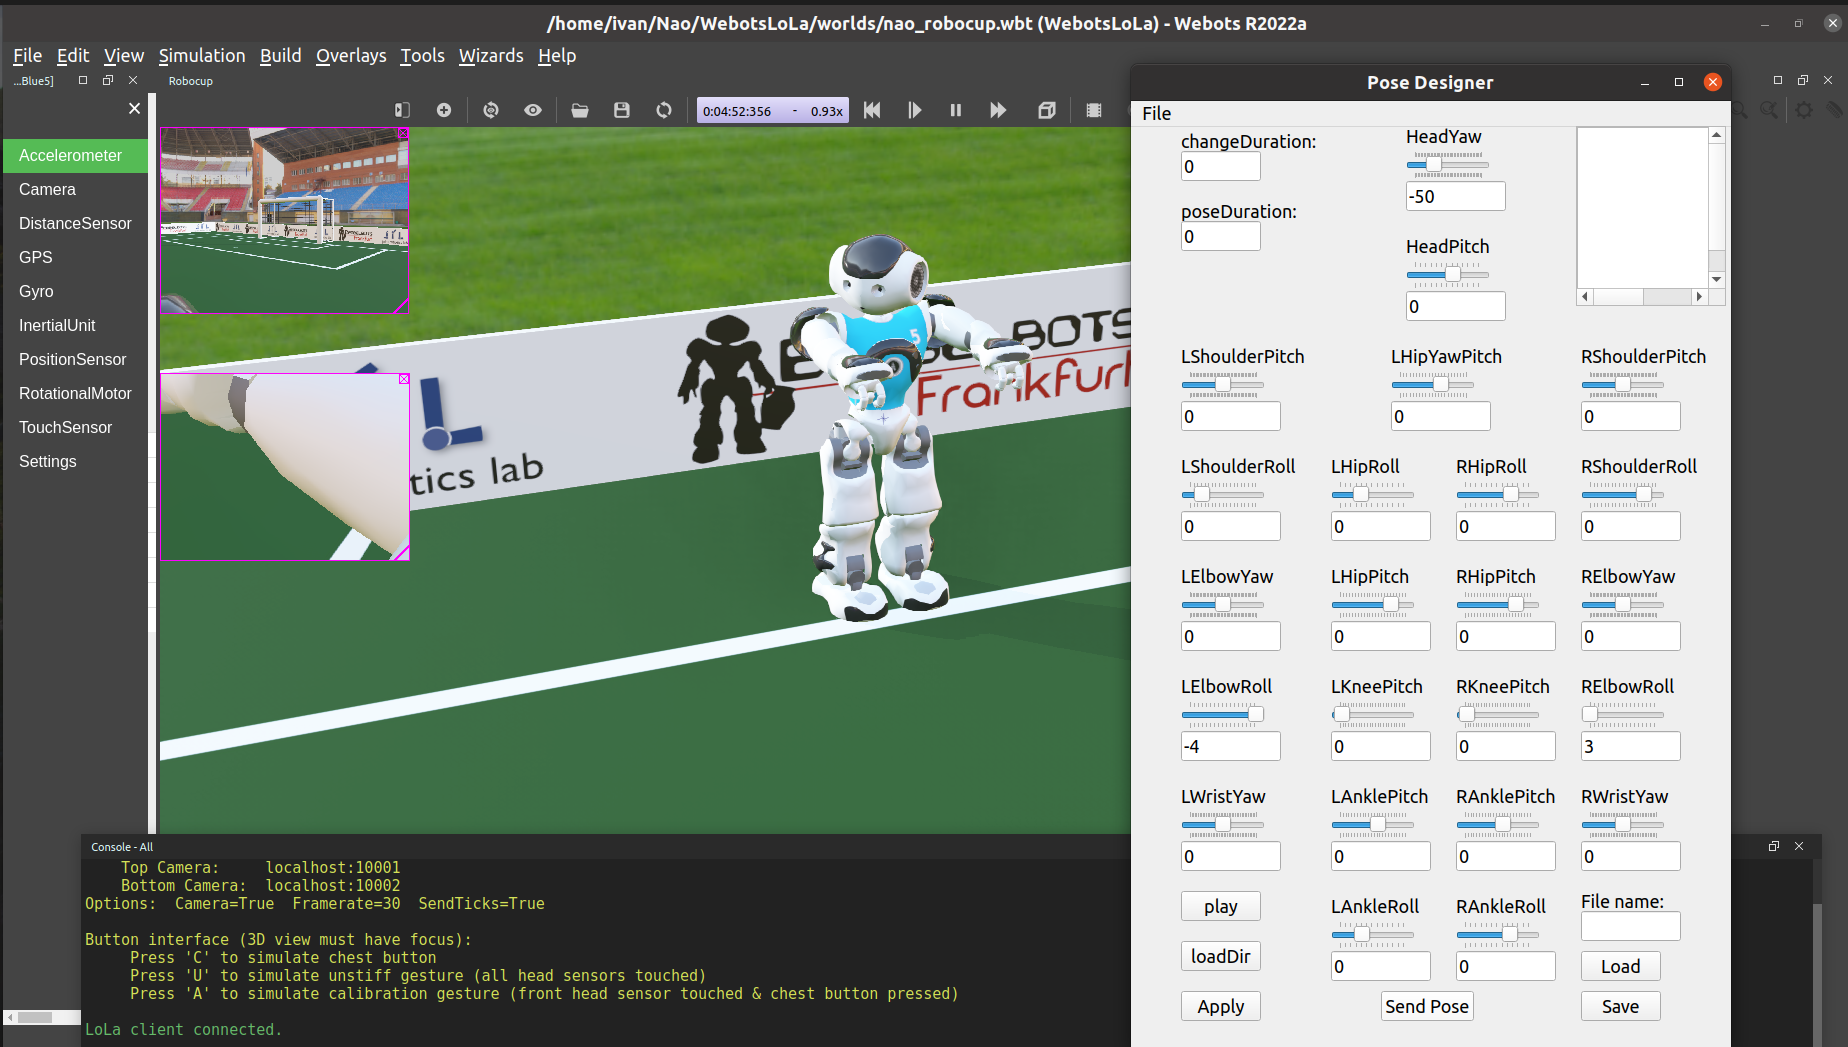
\includegraphics[width = 0.99\textwidth]{./images/secondTurn.png}
    \caption{Отправка второй позы.}
    \label{fig:my_label}
\end{figure}

Сохраним эту новую позу под названием \italic{pose2.txt}.
\begin{figure}[h!]
    \centering
    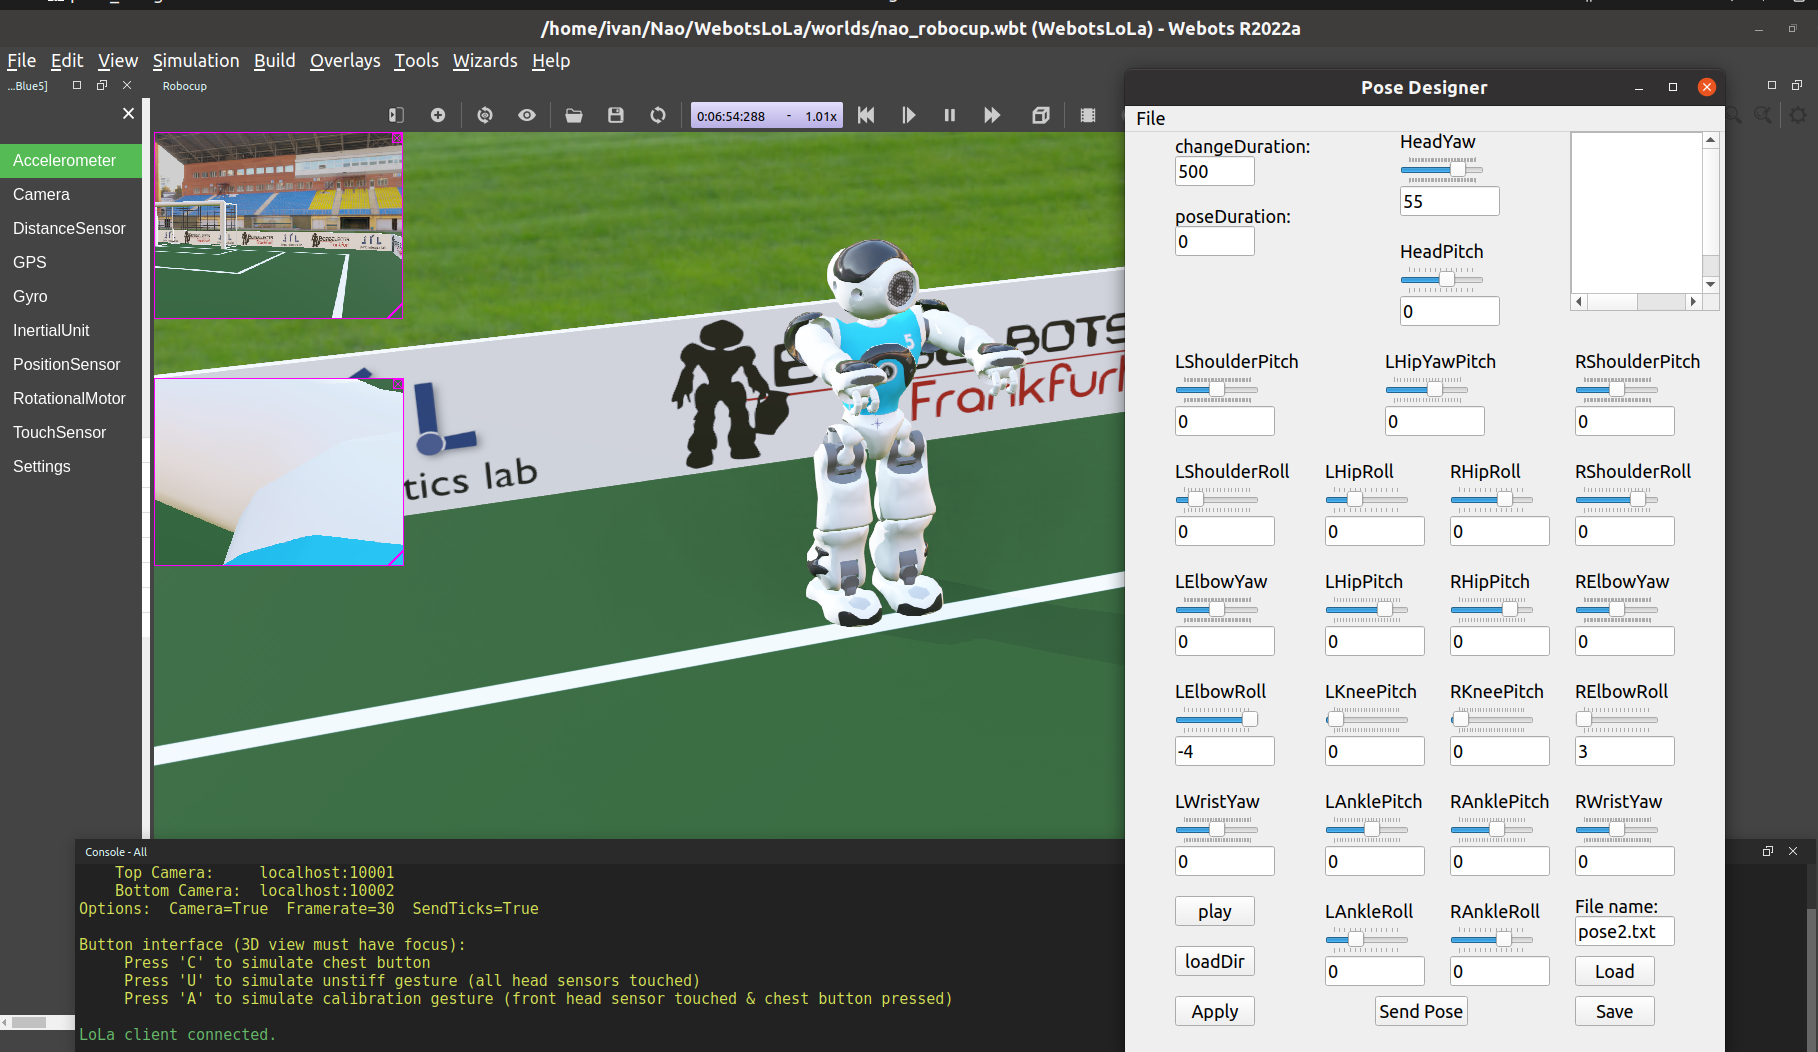
\includegraphics[width = 0.99\textwidth]{./images/secondSave.png}
    \caption{Сохранение второй позы.}
    \label{fig:my_label}
\end{figure}
\newpage
\subsection{Проигрывание поз}
Для проигрывание всех записаннызх(сохранённых) только что поз, необходимо, чтобы лни отобрализись в \hyperref[scroll]{области прокрутки}. Чтобы это произошло, нажимаем \hyperref[loadDir]{кнопку обновление директории загрузки}. После этого нажатие на \hyperref[play]{кнопку проигрывания} воспроизводит последовательно все позы из списка.
\begin{figure}[h!]
    \centering
    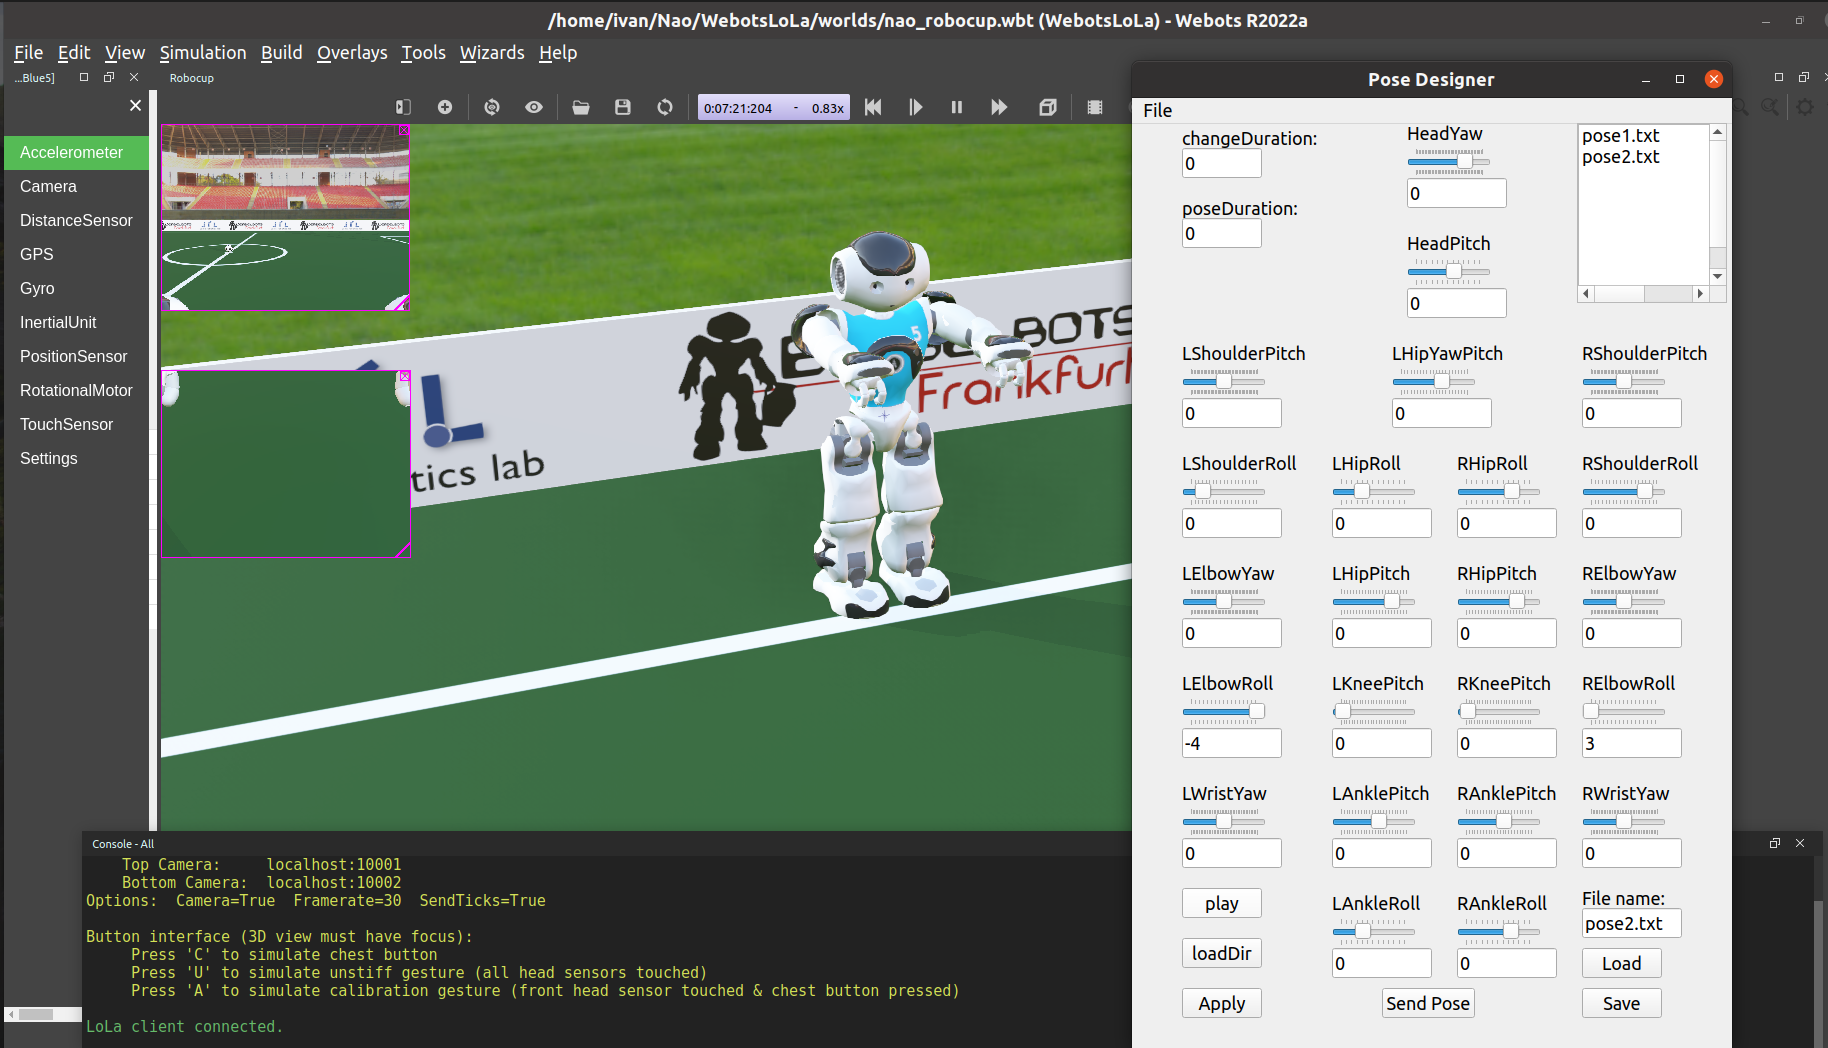
\includegraphics[width = 0.99\textwidth]{./images/playClick.png}
    \caption{Проигрывание поз.}
    \label{fig:my_label}
\end{figure}
\newpage
\section{Вид сообщений}
\label{messageView}
Поза - это файл в котором в столбик записаны значения в градусах каждого[25 - последнии два значения отвечают за сжатие кистей - в roboCup ненужны] соединения в диапозоне$\{ 0 \} \vee \mathbf{N}$. Последние два числа[26, 27 строчка] указывают на продолжительность[ms] позы и продолжительность[ms] перехода в следующую позу соответственно. Соединения расположенны в общепринятом порядке, который можно посмотреть на примере стандартной \italic{node} \href{https://github.com/ros-sports/nao_lola.git}{\textbf{nao\_lola}}.
\begin{figure}[h!]
    \centering
    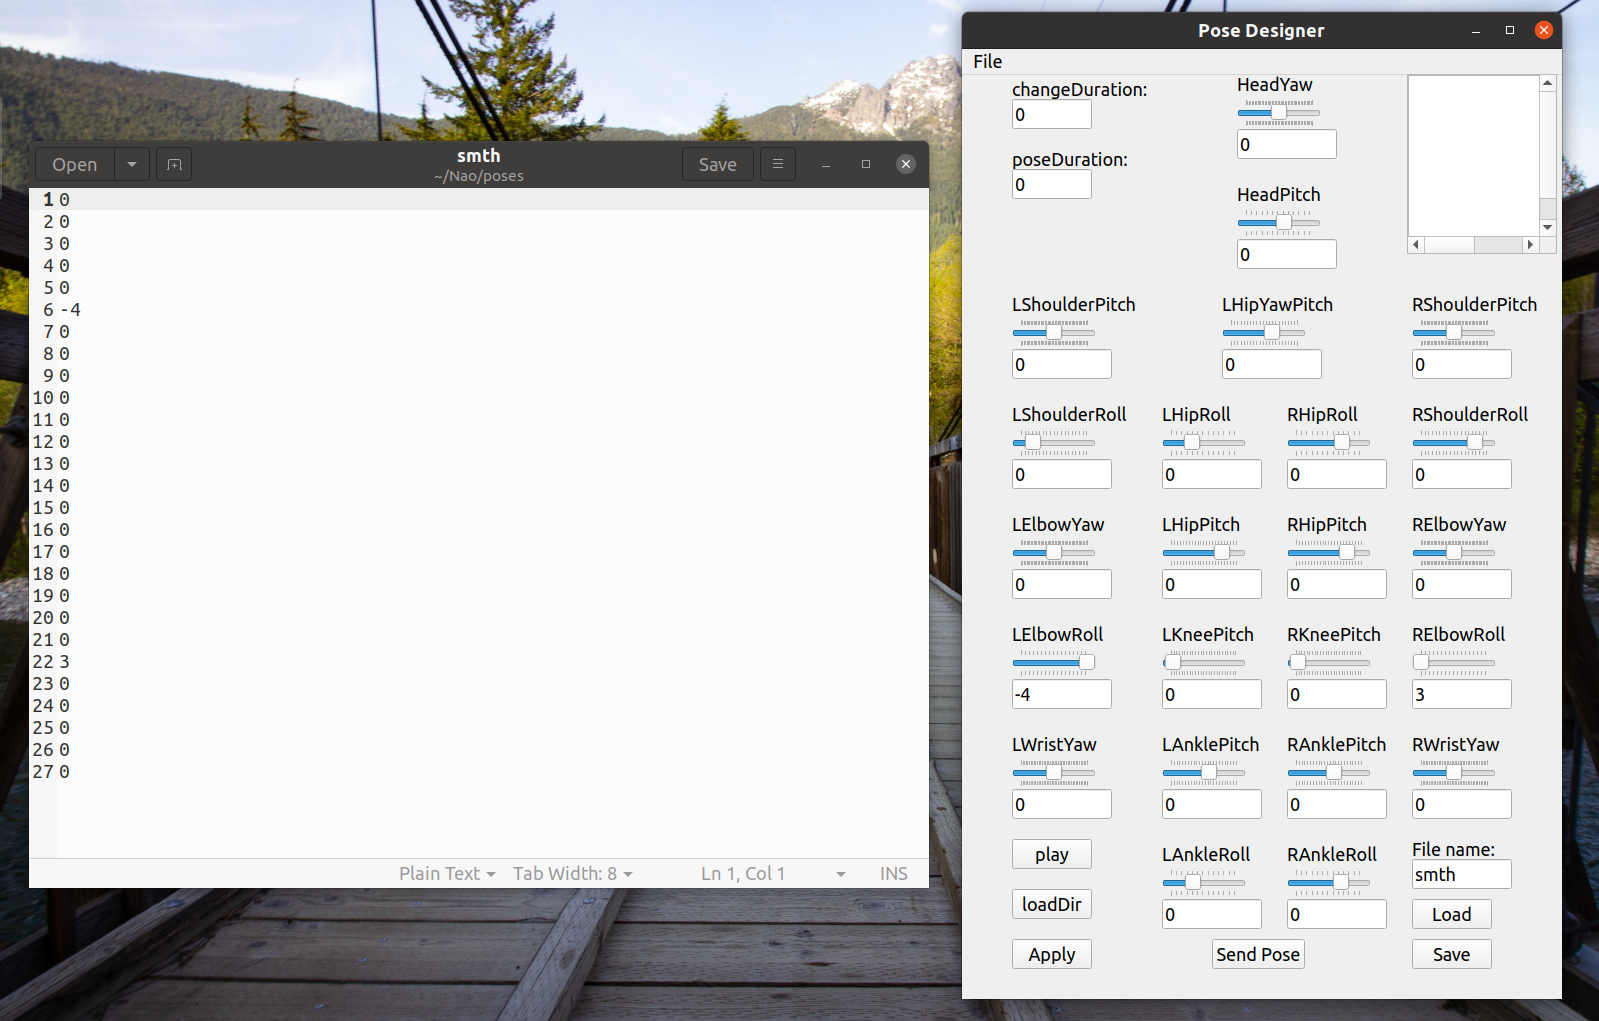
\includegraphics[width=0.99\textwidth]{images/message.png}
    \caption{Пример файла-позы с гачальными значениями при открытии приложения.}
    \label{fig:messageView}
\end{figure}
\end{document}
